\title{Numerical Analysis Final Assignment\\(in Portuguese)}
\author{Lucas Oliveira David \footnote{Universidade Federal de São Carlos, lucasolivdavid@gmail.com}\\[2cm]}
\author{Lucas Oliveira David\\[2cm]
	Universidade Federal de Sao Carlos\\[2cm]
	\textit{Numerical Analysis Class}\\
	Professor: Dr. Edgard A. Pimentel}
\date{\vfill \today}

\documentclass{article}

\usepackage{titlesec}
\usepackage{geometry}
\usepackage{graphicx}
\usepackage{caption}
\usepackage{subcaption}
\usepackage{mathtools}
\usepackage{amsmath}
\usepackage{amssymb}
\usepackage{amsfonts}
\usepackage{hyperref}
\usepackage{float}
\usepackage{wrapfig}
\usepackage{listings}
\usepackage[utf8]{inputenc}
\usepackage[english]{babel}

\graphicspath{assets}

\geometry{a4paper}

\begin{document}
	\begin{titlepage}
		\maketitle
	\end{titlepage}
	
	
	\section{Integração numérica}
	
	Seja $f \colon [1, 4] \subset \mathbb{R} \to \mathbb{R} \mid f(x) = \log x$ nossa função de interesse e $n=4$ o número de amostras coletadas no intervalo $[1, 4]$.
	
	\begin{align*}
		h = \frac{b - a}{n} = \frac{4-1}{4} = .75
	\end{align*}
	
	\subsection{Regra do trapézio}
		\begin{align*}
		\int_{1}^{4} \log x dx &\approx \frac{h}{2} [\log x_0 + \log x_n + 2 \sum_{i=1}^{n-1}  \log x_i] \text{, where } x_i = x_0+hi. \\
		&= \frac{.75}{2} [\log 1 + \log 4 + 2(\log 1.75 + \log 2.5 + \log 3.25)] \\
		&= .375 [0 + 1.386294361 + 2(0.559615788 + 0.916290732 + 1.178654996)] \\
		&= .375[6.695417393] \\
		&= 2.510781522
		\end{align*}

	\subsection{Regra de Simpson}
		\begin{align*}
		\int_{1}^{4} \log x dx &\approx \frac{h}{3} [\log x_0 + \log x_n + 2 \sum_{i=1}^{n-1}  \log x_i + 2 \sum_{i=0}^{\frac{n}{2}-1} x_{2i+1}] \text{, where } x_i = x_0+hi. \\
		&= \frac{.75}{3} [6.695417393 + 2(0.559615788 + 1.178654996)] \\
		&= \frac{.75}{3}[10.171958961] \\
		&= 2.54298974
		\end{align*}

	\newpage
	\section{Solução numérica para equações diferenciais ordinárias}
	
	Seja $y \colon [0, .5] \in \mathbb{R}$ e $n=5$ iterações, estime o valor de  $y_5$ para o problema de valores iniciais abaixo:
	\begin{align*}
		P &= \begin{cases}
		\dot{y} = y +xy \\
		y_0 = 1
		\end{cases}
	\end{align*}

	\subsection{Método explicito de Euler}
		\begin{align*}
			h &= \frac{b-a}{n} = \frac{.5-0}{5} = .1 \\
			y_{n+1} &= y_n + hf(y_n, x_n) \\
			y_{n+1} &= y_n + .1 (y_n + x_n y_n) \\
			y_{n+1} &= y_n[1 + .1 + .1x_n]
		\end{align*}
		\begin{table}[H]
			\centering
			\begin{tabular}{|c|c|c|}
				\hline
				$n$ & $x_n$ & $y_n$ \\\hline
				0       &  0    & 1      \\\hline
				1       & .1    & 1.1  \\\hline
				2       & .2    & 1.221 \\\hline
				3       & .3    & 1.36752 \\\hline
				4       & .4    & 1.5452976 \\\hline
				5       & .5    & 1.761639264 \\\hline
			\end{tabular}
			\captionsetup{justification=centering}
			\caption{Iterações do método de Euler explícito.}
		\end{table}
		\begin{align*}
		\therefore
		y_5 = 1.761639264
		\end{align*}
	
	\subsection{Método implícito de Euler}
	\begin{align*}
		y_{n+1} &= y_n + hf(y_{n+1}, x_{n+1}) \\
		&= y_n + .1 (y_{n+1} + x_{n+1} y_{n+1}) \\
		&= y_n + .1 y_{n+1} (1 + x_{n+1}) \\
		&= y_n + .1 y_{n+1} (x_{n} + 1.1) \\
		&\iff \\
		y_{n+1} -.1 y_{n+1} (x_{n} + 1.1) &= y_n \\
		y_{n+1}[1 -.1 (x_{n} + 1.1)] &= y_n \\
		y_{n+1} &= \frac{y_n}{1 -.1 (x_{n} + 1.1)} \\
		y_{n+1} &= \frac{y_n}{.89 -.1x_{n}} \\
	\end{align*}
	\begin{table}[H]
		\centering
		\begin{tabular}{|c|c|c|}
			\hline
			$n$ & $x_n$ & $y_n$          \\\hline
			0       &  0    & 1      				      \\\hline
			1       & .1    & 1.123595506 \\\hline
			2       & .2    & 1.276813075 \\\hline
			3       & .3    & 1.467601235 \\\hline
			4       & .4    & 1.706513064 \\\hline
			5       & .5    & 2.007662428 \\\hline
		\end{tabular}
		
		\captionsetup{justification=centering}
		\caption{Iterações do método Euler implícito.}
	\end{table}
	\begin{align*}
	\therefore
	y_5 = 2.007662428
	\end{align*}
	
	\subsection{Método de Heun}
		\begin{align*}
			y_{n+1} &= y_n +  h \frac{1}{2} [f(y_n, x_n) + f(y_{n+1}, x_{n+1})] \\
			y_{n+1} &= y_n + \frac{1}{20}[y_n + x_n y_n + y_{n+1} +  x_{n+1} y_{n+1}] \\
			y_{n+1} -\frac{y_{n+1} + y_{n+1} x_{n+1}}{20} &= y_n + \frac{1}{20}(y_n + y_n x_n) \\
			y_{n+1} \frac{19-x_{n+1}}{20}  &= \frac{21 y_n + x_n y_n}{20} \\
			y_{n+1} &= \frac{21 y_n + x_n y_n}{18.9 - x_n} \\
			y_{n+1} &= \frac{y_n (21 + x_n)}{18.9 - x_n} \\
		\end{align*}
		\begin{table}[H]
			\centering
			\begin{tabular}{|c|c|c|}
				\hline
				$n$ & $x_n$ & $y_n$ \\\hline
				0       &  0    & 1      				      \\\hline
				1       & .1    & 1.111111111 \\\hline
				2       & .2    & 1.247044917 \\\hline
				3       & .3    & 1.413762152 \\\hline
				4       & .4    & 1.61898569 \\\hline
				5       & .5    & 1.872772636 \\\hline
			\end{tabular}
			
			\captionsetup{justification=centering}
			\caption{Iterações do método Euler implícito.}
		\end{table}
		\begin{align*}
		\therefore
		y_5 = 1.872772636
		\end{align*}

	\newpage
	\section{Principal Component Analysis utilizando Decomposição de valor singular (SVD)}
	Seja $K = [k_{ij}]_{2 \times n}$ um conjunto de dados com $n$ amostras e duas características. O conjunto segue uma certa distribuição, como ilustrado na figura abaixo:
	
	\begin{figure}[H]
		\centering
		\captionsetup{justification=centering}
		
		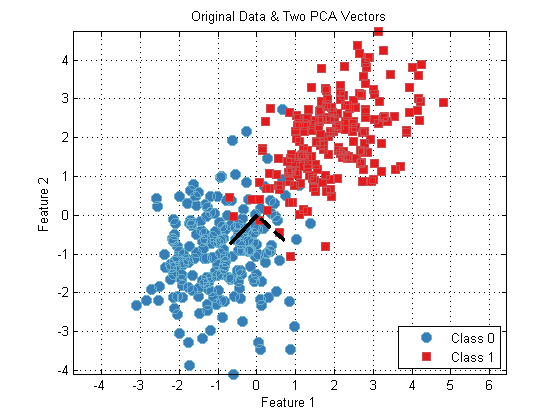
\includegraphics[width=.8\linewidth]{assets/k}
		\caption{O conjunto de dados $K \subset \mathbb{R}^2$.}
		\label{fig:datasetk}
	\end{figure}
	
	Redução dimensional é um assunto amplamente abordado em multiplos contextos (e.g., estatístico, computacional) a fim de reduzir a necessidade por recursos computacionais ou melhoramento de visualização. Consiste em, a partir de um conjunto $X$, encontrar um conjunto $Y$ de menor dimensionalitade tal que a perca de informação seja mínima.
	
	Uma das técnicas mais conhecidas empregadas na redução dimensional é Principal Component Analysis (PCA), descrita abaixo:
	\begin{description}
		\item[Identificando as componentes principais]
		Se o conjunto de dados está centrado na origem do espaço (como o da figura 1), as componentes principais (vetores em preto) são exatamente os autovetores da matrix de covariância das características ($\frac{1}{n} K K^T$), multiplicados pelas raizes de seus seus respectivos autovalores:
		\begin{align*}
			K &= U \Sigma V^T \\
			\Sigma_X &= \frac{1}{n} K K^T \\
			\implies \\
			\Sigma_X &= \frac{1}{n} (U \Sigma V^T) (U \Sigma V^T)^T = \frac{1}{n} U \Sigma^2 U^T
		\end{align*}
		
		Singular Value Decomposition (SVD) pode ser utilizada para extrair tais autovetores/valores!
		
		\item[Seleção de PCs]
		
		Todos os autovetores são vetores unitários, e a variância das amostras em uma determinada direção $v_i$ é dada pelo autovalor associado $\lambda_i$. Portanto os autovetores (colunas de $U$) podem ser ordenados descrecentemente usando $|\lambda_i|$ como valor de comparação; finalmente, componentes (colunas de $U$) com baixa variancia podem ser eliminados.
		
		\item[Projetando amostras do espaço original para o reduzido]
		Observe que os autovetores formam uma base, logo $Vy = x$, onde $x \in X, y \in Y$. Portanto, a matrix $V^{-1}$ é a matrix de projeção de $X$ para $Y$, mas $V$ é ortonormal (propriedade de SVD + fato de reordenar colunas não alterar a ortogonalidade de uma matriz), então
		\begin{align*}
			V^{-1} = V^T \implies V^T x = y
		\end{align*}
	\end{description}
	
	A figura abaixo ilustra a aplicação do PCA sobre um conjunto de dados $R$:
	
		\begin{figure}[H]
			\centering
			\captionsetup{justification=centering}
			
			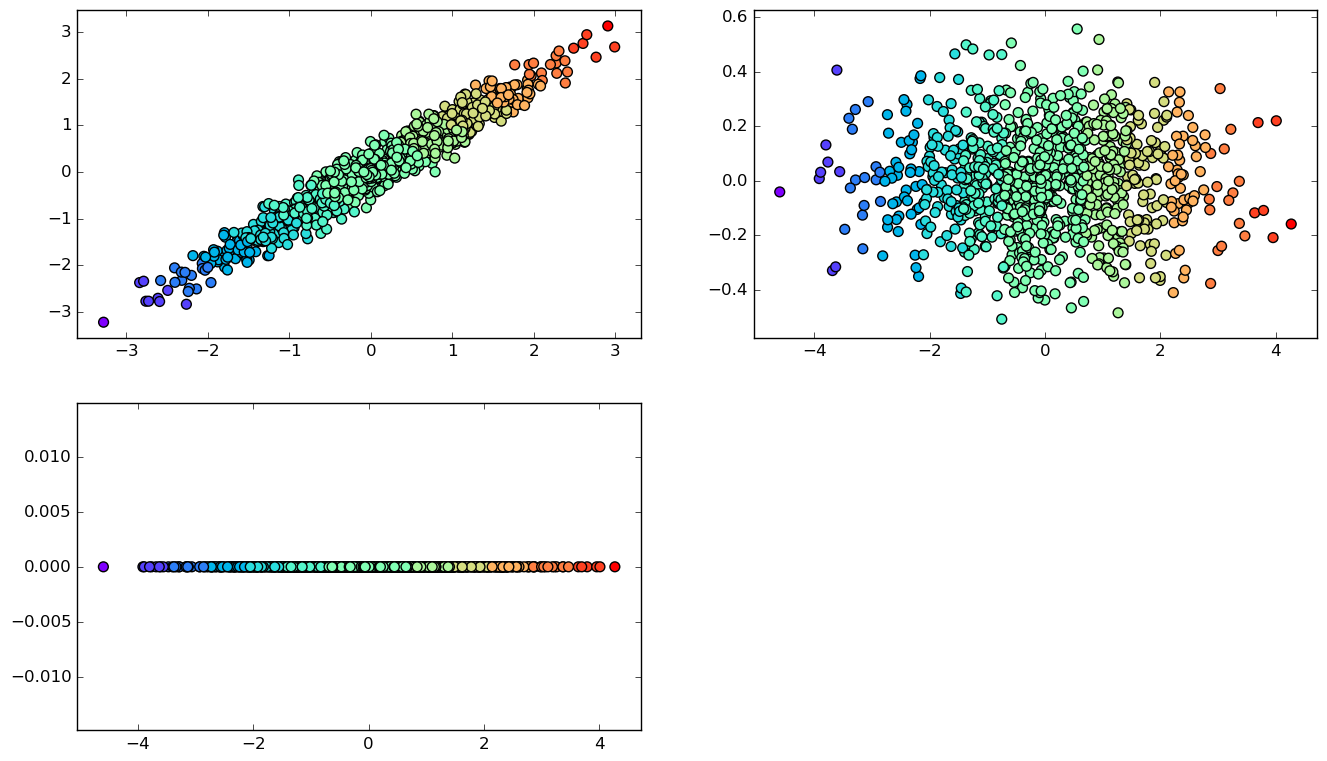
\includegraphics[width=\linewidth]{assets/r}
			\caption{O conjunto de dados $R \subset \mathbb{R}^2$ e sua redução para o $\mathbb{R}^2$ e $\mathbb{R}$, respectivamente.}
			\label{fig:datasetr}
		\end{figure}
		
\end{document}
